% ----------------
% 节: 附录A scu 宏包
% ----------------
\section{附录A}
\subsection{scu 主题选项预览}
\begin{frame}{Info.}
	\textbf{本小节将展示部分 scu 主题选项的预览效果.}
	\begin{multicols}{2}
		\begin{itemize}
			\item \myestablish{v1.3e}{2024/10/31}
			\item \myupdate{v1.3e}{2024/10/31}
		\end{itemize}
	\end{multicols}
	注: 本小节仅对部分主题参数进行了演示, 您可点击标题栏 \texttt{BACK} 字样返回对应的宏包参数说明处.\par
	\mycopyright
\end{frame}

\begin{frame}{颜色主题预览 \scugoback{back:ColorDisplay}{BACK}}\label{goto:ColorDisplay}
  \structure{\cmd{usetheme}\oarg*{ColorDisplay=\Arg{value}}\marg*{scu}}
	\begin{columns}[T, onlytextwidth]
    \begin{column}{.5\textwidth}
      \structure{锦锈红} \Arg{value}\texttt{=JXred}
      \begin{figure}[h]
        \centering
        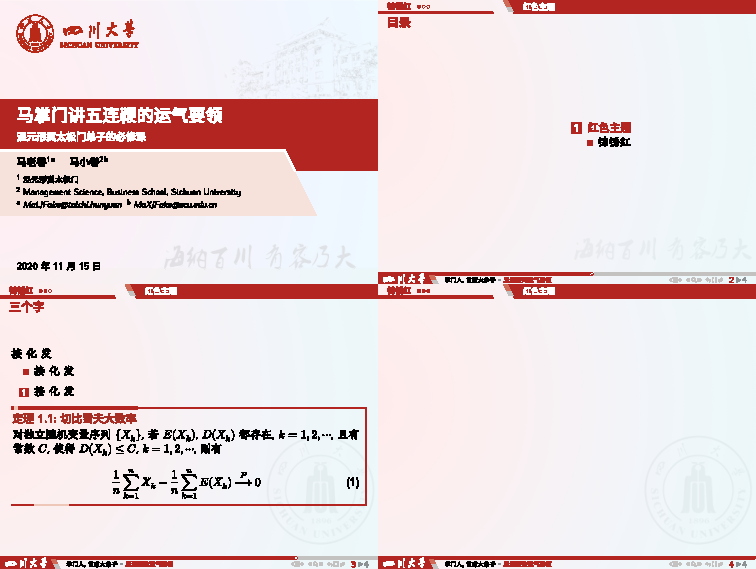
\includegraphics[width=\columnwidth]{manual-sec/manual-demo/appendix-themescu-ColorDisplay-1.pdf}
      \end{figure}
    \end{column}
    \begin{column}{.5\textwidth}
      \structure{宝石蓝} \Arg{value}\texttt{=BSblue}
      \begin{figure}[h]
        \centering
        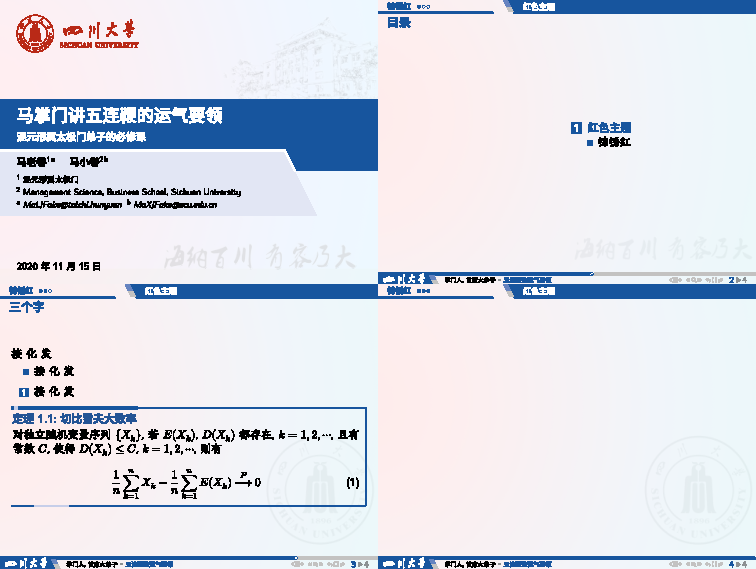
\includegraphics[width=\columnwidth]{manual-sec/manual-demo/appendix-themescu-ColorDisplay-2.pdf}
      \end{figure}
    \end{column}
  \end{columns}
\end{frame}

\begin{frame}{小节迷你帧预览 \scugoback{back:Miniframes}{BACK}}\label{goto:Miniframes}
  \vspace*{-6ex}
  \begin{figure}[h]
    \begin{tikzpicture}
      \node[anchor=south west] (img) at (0,10pt) {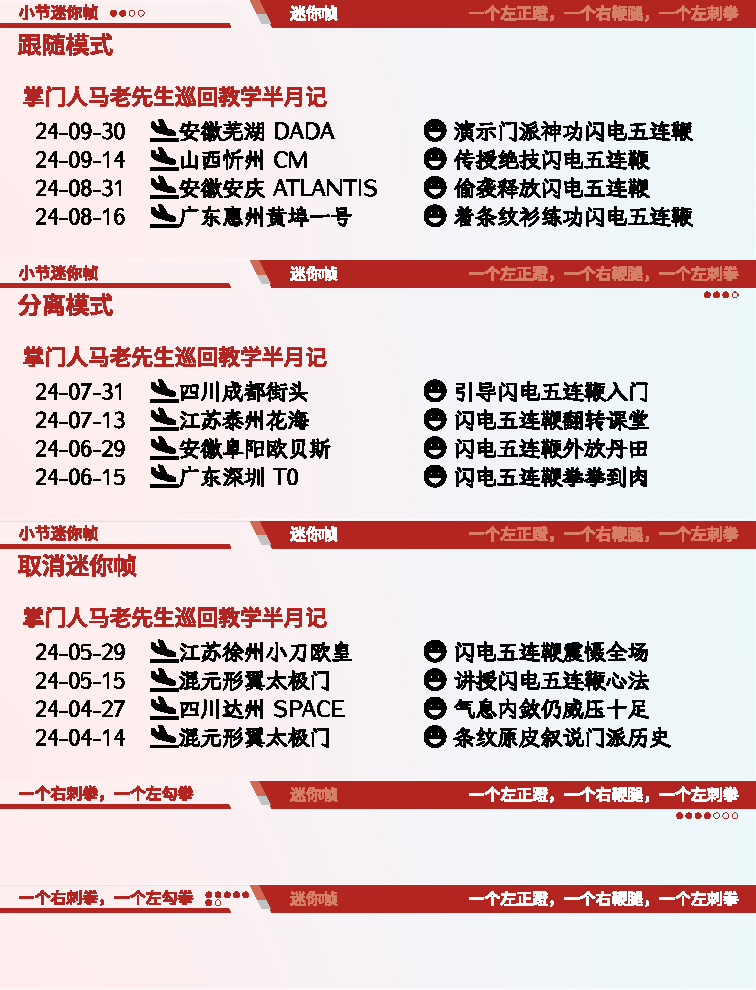
\includegraphics[height=.88\textheight]{manual-sec/manual-demo/appendix-themescu-Miniframes.pdf}};
      \node[anchor=west] at (8, 211.4pt) {\structure{\cmd{usetheme}\oarg*{Miniframes=\Arg{value}}\marg*{scu}}};
      % --------- First ----------
      \def\xFir{28.8pt}
      \def\yFir{211.4pt}
      \draw[scublue, thin] (\xFir-6pt, \yFir-2pt) rectangle (\xFir+6pt, \yFir+2pt); % 以 (x, y) 为中心的框
      \draw[scublue, thin] (\xFir+6pt, \yFir-2pt) -- (\xFir+28pt, \yFir-13pt); % 斜线
      \draw[scublue, thin] (\xFir+28pt, \yFir-13pt) -- (8, \yFir-13pt); % 水平线
      \node[anchor=west] (NodeOne) at (8, \yFir-13pt) {\structure{迷你帧跟随} \Arg{value}\texttt{=follow}};
      \node[anchor=west] at ([yshift=-12pt]NodeOne.west) {迷你帧跟随当前小节标题(如此处为“小节迷你帧”)};
      % ---------- Second ----------
      \def\xSec{149.5pt}
      \def\ySec{154.2pt}
      \draw[scublue, thin] (\xSec-6pt, \ySec-2pt) rectangle (\xSec+6pt, \ySec+2pt); % 以 (x, y) 为中心的框
      \draw[scublue, thin] (\xSec+6pt, \ySec) -- (8, \ySec); % 水平线
      \node[anchor=west] (NodeTwo) at (8, \ySec) {\structure{迷你帧分离} \Arg{value}\texttt{=separate}};
      \node[anchor=west] at ([yshift=-12pt]NodeTwo.west) {迷你帧与小节标题分离(位于节导航栏下方且右侧对齐)};
      % ---------- Third ----------
      \def\xThiO{28.8pt}
      \def\yThiO{105.5pt}
      \draw[scublue, thin] (\xThiO-6pt, \yThiO-2pt) rectangle (\xThiO+6pt, \yThiO+2pt); % 以 (x, y) 为中心的框
      \draw[scublue, thin] (\xThiO+6pt, \yThiO-2pt) -- (\xThiO+28pt, \yThiO-13pt); % 斜线
      \draw[scublue, thin] (\xThiO+28pt, \yThiO-13pt) -- (8, \yThiO-13pt); % 水平线
      \def\xThiT{149.5pt}
      \def\yThiT{101.3pt}
      \draw[scublue, thin] (\xThiT-6pt, \yThiT-2pt) rectangle (\xThiT+6pt, \yThiT+2pt); % 以 (x, y) 为中心的框
      \draw[scublue, thin] (\xThiT+6pt, \yThiT-2pt) -- (\xThiT+19.6pt, \yThiT-8.8pt); % 斜线
      \node[anchor=west] (NodeThree) at (8, \yThiO-13pt) {\structure{取消迷你帧} \Arg{value}\texttt{=negate}};
      \node[anchor=west] at ([yshift=-12pt]NodeThree.west) {页眉上无迷你帧显示};
      % ---------- Forth ----------
      \def\xForO{146.6pt}
      \def\yForO{48.2pt}
      \draw[scublue, thin] (\xForO-8pt, \yForO-2pt) rectangle (\xForO+8pt, \yForO+2pt); % 以 (x, y) 为中心的框
      \draw[scublue, thin] (\xForO+8pt, \yForO-2pt) -- (\xForO+20pt, \yForO-8pt); % 斜线
      \def\xForT{49pt}
      \def\yForT{31.4pt}
      \draw[scublue, thin] (\xForT-6pt, \yForT-2.8pt) rectangle (\xForT+6pt, \yForT+2.8pt); % 以 (x, y) 为中心的框
      \draw[scublue, thin] (\xForT+6pt, \yForT+2.8pt) -- (\xForT+18pt, \yForT+8.8pt); % 斜线
      \draw[scublue, thin] (\xForT+18pt, \yForT+8.8pt) -- (8, \yForT+8.8pt); % 水平线
      \node[anchor=west, align=left, yshift=-4pt] at (8, \yForT+8.8pt) {自v1.3e起,迷你帧支持点击跳转\\若小节中页面数量过多且设置迷你帧跟随小节标题时\\\alert{迷你帧可自适应换行}\\反之设置迷你帧与小节标题分离则单行显示};
    \end{tikzpicture}
  \end{figure}
  \vspace*{-6ex}
\end{frame}

\begin{frame}{导航工具栏详情 \scugoback{back:NavigationTool}{BACK}}\label{goto:NavigationTool}
  \structure{\cmd{usetheme}\oarg*{NavigationTool=\Arg{value}}\marg*{scu}}\vspace*{-2.5ex}
  \begin{figure}[h]
    \centering
    
\includegraphics[width=\textwidth]{manual-sec/manual-demo/appendix-themescu-NavigationTool.pdf}
  \end{figure}

  \structure{小节及小节跳转工具} 标记为1 - \alert{\hskip.4pt\setfontscu{5}\faCaretLeft\hskip1.6pt\faStream\hskip1.6pt\faCaretRight}\vspace*{1ex}

  \begin{tabular}{l>{\raggedright\arraybackslash}p{.02\textwidth}>{\raggedright\arraybackslash}p{.35\textwidth}l}
    核心工具 & {\setfontscu{5}\faStream} & 前往当前小节开始 & -\\
    附加工具 & {\setfontscu{5}\faCaretLeft} & 前往上一小节末尾 & -\\
    附加工具 & {\setfontscu{5}\faCaretRight} & 前往下一小节开始 & -\\
  \end{tabular}\vspace*{1ex}

  \structure{查询及首尾跳转工具} 标记为2 - \alert{\hskip.4pt\setfontscu{5}\faCaretLeft\hskip-.05em\faCaretLeft\hskip1.6pt\setfontscu{4.5}\faSearch\hskip1.6pt\setfontscu{5}\faCaretRight\hskip-.05em\faCaretRight}\vspace*{1ex}

  \begin{tabular}{l>{\raggedright\arraybackslash}p{.02\textwidth}>{\raggedright\arraybackslash}p{0.35\textwidth}l}
    核心工具 & {\setfontscu{4.5}\faSearch} & 查找(需要使用Adobe Acrobat) & Acrobat快捷键: Ctrl + F\\
    附加工具 & {\setfontscu{5}\faCaretLeft\hskip-.05em\faCaretLeft} & 前往初始页(不包含附录) & -\\
    附加工具 & {\setfontscu{5}\faCaretRight\hskip-.05em\faCaretRight} & 前往结尾页(不包含附录) & -\\
  \end{tabular}\vspace*{1ex}

  \structure{放映及历史跳转工具} 标记为3 - \alert{\hskip.4pt\setfontscu{4.5}\faReply\hskip1.6pt\setfontscu{5}\faExpand\hskip1.6pt\setfontscu{4.5}\reflectbox{\faReply}}\vspace*{1ex}

  \begin{tabular}{l>{\raggedright\arraybackslash}p{.02\textwidth}>{\raggedright\arraybackslash}p{0.35\textwidth}l}
    核心工具 & {\setfontscu{5}\faExpand} & 全屏或退出全屏(需要使用Adobe Acrobat) & Acrobat快捷键: Ctrl + L\\
    附加工具 & {\setfontscu{4.5}\faReply} & 前往上一视图(需要使用Adobe Acrobat) & Acrobat快捷键: Alt + 向左箭头\\
    附加工具 & {\setfontscu{4.5}\reflectbox{\faReply}} & 前往下一视图(需要使用Adobe Acrobat) & Acrobat快捷键: Alt + 向右箭头\\
  \end{tabular}
\end{frame}

\subsection{scu 主题项目结构}
\begin{frame}{Info.}
	\textbf{本小节将展示 scu 主题的项目结构.}
	\begin{multicols}{2}
		\begin{itemize}
			\item \myestablish{v1.3e}{2024/10/31}
			\item \myupdate{v1.3e}{2024/10/31}
		\end{itemize}
	\end{multicols}
	注: 自 \textcolor{scugreen}{v1.3e (2024/10/31)} 起, 本小节已替代手册中\alert{\textbf{使用注意}}小节的\alert{项目结构}板块.\par
	\mycopyright
\end{frame}
\begin{frame}{main 分支文件结构 \scugoback{back:BranchMain}{BACK}}\label{goto:BranchMain}
  从 release 中下载的版本也具有如下的文件结构.
  \begin{multicols}{2}
    \setlength{\DTbaselineskip}{10pt}
    \dirtree{%
    .1 \alert{SCU Beamer Theme}/.
    .2 fonts/\DTcomment{\alert{字体存放}[资源]}.
    .2 image/\DTcomment{\alert{图像存放}[资源]}.
    .2 mintedbuild/\DTcomment{\alert{minted 缓存}[缓存]}.
    .2 resources/\DTcomment{\alert{\textbf{scu 主题素材}}[主题]}.
    .3 SCUbuilding.png\DTcomment{\text{建筑}[主题]}.
    .3 SCUlogo\_name.pdf\DTcomment{\text{logo + 校名}[主题]}.
    .3 SCUname.pdf\DTcomment{\text{校名}[主题]}.
    .3 SCUverify.png\DTcomment{\text{校训}[主题]}.
    .3 background.png.
    .3 backgroundofsubsectiontocpage.png.
    .3 backgroundoftitlepage(Empty).png.
    .3 backgroundoftitlepage(Light).png.
    .3 backgroundoftitlepage.png.
    .2 sourcecode/\DTcomment{\alert{代码存放}[资源]}.
    }
    \dirtree{%
    .1 \alert{SCU Beamer Theme}/.
    .2 beamercolorthemescu.sty\DTcomment{\alert{\textbf{颜色主题}}[主题]}.
    .2 beamerinnnerthemescu.sty\DTcomment{\alert{\textbf{内部主题}}[主题]}.
    .2 beamerouterthemescu.sty\DTcomment{\alert{\textbf{外部主题}}[主题]}.
    .2 beamerthemescu.sty\DTcomment{\alert{\textbf{scu核心主题}}[主题]}.
    .2 .gitignore.
    .2 LICENSE.
    .2 README.md.
    .2 main.tex\DTcomment{\alert{cn模式tex文件}[示例]}.
    .2 main.pdf\DTcomment{\alert{cn模式pdf文件}[示例]}.
    .2 main-en.tex\DTcomment{\alert{en模式tex文件}[示例]}.
    .2 main-en.pdf\DTcomment{\alert{en模式pdf文件}[示例]}.
    .2 manual.pdf\DTcomment{\alert{\textbf{用户手册}}[手册]}.
    .2 ref.bib\DTcomment{\alert{\textbf{文献库}}[资源]}.
    }
  \end{multicols}
\end{frame}

\begin{frame}{manual 分支文件结构 \scugoback{back:BranchManual}{BACK}}\label{goto:BranchManual}
  如下的示例演示资源中,pdf文件并不完全是tex直接编译所得,而是编译后经过inkscape拼接、裁剪和压缩生成.
  \begin{multicols}{2}
    \setlength{\DTbaselineskip}{10pt}
    \dirtree{%
    .1 \alert{SCU Beamer Theme Manual}/.
    .2 manual-sec/\DTcomment{\alert{手册分节tex文件}[章节]}.
    .3 manual-demo/\DTcomment{\alert{手册中示例演示资源}[演示]}.
    .4 \text{...}.tex\DTcomment{\alert{示例tex文件}[演示]}.
    .4 \text{...}.pdf\DTcomment{\alert{示例pdf文件}[演示]}.
    .3 base-settings.tex\DTcomment{\alert{基础设置}[章节]}.
    .3 appendix-themescu.tex\DTcomment{\alert{附录A}[章节]}.
    }\columnbreak
    \dirtree{%
    .1 \alert{SCU Beamer Theme Manual}/.
    .2 manual.tex\DTcomment{\alert{用户手册tex文件}[手册]}.
    .2 manual.pdf\DTcomment{\alert{用户手册pdf文件}[手册]}.
    }
  \end{multicols}
\end{frame}